\documentclass[tikz,border=2pt]{standalone}
\usepackage{tikz}
\usetikzlibrary{positioning}
\begin{document}
	\begin{tikzpicture}[
	main/.style={rectangle, rounded corners, text centered, text width=3cm, draw=black},
	aux/.style={}
	]	
	
	\node (project) [main] {Project};
	

		
		\node (sim) [main, below=of project] {Simulation};
			\node (aux2) [aux, below=of sim] {};
			\node (mathsim) [main, left=1.5cm of aux2] {Mathematical Simulation};
			\node (visualsim) [main, right=1.5cm of aux2] {Visual simulation};
				\node (aux6) [aux, below=of visualsim] {};
				\node (simulatequad) [main, left=of aux6] {Simulate quad};
				\node (simulateenvironm) [main, right=of aux6] {Simulate environment \& obstacles};
				
		\node (multiagent) [main, left=10cm of sim] {Multi-agent case};
				\node (aux10) [aux, below=of multiagent] {};	
				\node (multiagentcontrol) [main, right=2.5cm of aux10] {Control};
				\node (multiagentmodelling) [main, left=2.5cm of aux10] {Modelling};
				
		\node (control) [main, left=12 cm of multiagent] {Quad Control};
			\node (aux8) [aux, below=of control] {};
			\node (navigation) [main, right=3cm of aux8] {Navigation};
				\node (aux5) [aux, below=of navigation] {};
				\node (potfields) [main, left=of aux5] {Potential fields};
				\node (astar) [main, right=of aux5] {A* and others};
			\node (tracking) [main, left=3cm of aux8] {Tracking};
				\node (aux9) [aux, below=of tracking] {};
				\node (timetraj) [main, left=of aux9] {Time trajectory};
				\node (stabilization) [main, right=of aux9] {Stabilization};
		
		\node (mod) [main, left=10cm of control] {Modelling};
			\node (aux4) [aux, below=of mod] {};	
			\node (quadmod) [main, left=2.5cm of aux4] {Quad};
				\node (aux7) [aux, below=of quadmod] {};
				\node (dynamics) [main, right=of aux7] {Dynamics};	
				\node (kinematics) [main, left=of aux7] {Kinematics};
			\node (sensorsmod) [main, right=of aux4] {Sensors};
						
		\node (lit) [main, left=18cm of mod] {Literature};
			\node (sensorslit) [main, below=of lit] {Sensors};
				\node (sensorsjour) [main, below=of sensorslit] {Model \& use of sensors in drones in IEEE journals};
			\node (modlit) [main, left=3cm of sensorslit] {Quads modelling};
				\node (aux3) [aux, below=of modlit] {};
				\node(weighandforces)[main, left=of aux3] {Quad weight \& forces model in IEEE journals};
				\node(movement)[main, right=of aux3] {Quad movement model in IEEE journals};
			\node (trackinglit) [main, right=of sensorslit] {Tracking};
				\node (trackjour) [main, below=of trackinglit] {Read articles in IEEE journals};
		
		\node (results) [main, right=2cm of sim] {Results and conclusions};	
		\node (rep) [main, right=of results] {Report};
		\node (peerrev) [main, right=of rep] {Peer-Review};
		\node (presentation) [main, right=of peerrev] {Presentation};	

	\draw [-latex] (project.south)--++(0,-.3)-| (lit.north);
	\draw [-latex] (project.south)--++(0,-.3)-| (mod.north);
	\draw [-latex] (project.south)--++(0,-.3)-| (sim.north);
	\draw [-latex] (project.south)--++(0,-.3)-| (results.north);
	\draw [-latex] (project.south)--++(0,-.3)-| (rep.north);
	\draw [-latex] (project.south)--++(0,-.3)-| (peerrev.north);
	\draw [-latex] (project.south)--++(0,-.3)-| (control.north);
	\draw [-latex] (project.south)--++(0,-.3)-| (multiagent.north);
	\draw [-latex] (project.south)--++(0,-.3)-| (presentation.north);
	
	\draw [-latex] (lit.south)--++(0,-.3)-| (modlit.north);
	\draw [-latex] (lit.south)--++(0,-.3)-| (sensorslit.north);
	\draw [-latex] (lit.south)--++(0,-.3)-| (trackinglit.north);
	
	\draw [-latex] (mod.south)--++(0,-.3)-| (quadmod.north);
	\draw [-latex] (mod.south)--++(0,-.3)-| (sensorsmod.north);
	
	\draw [-latex] (control.south)--++(0,-.3)-| (navigation.north);
	\draw [-latex] (control.south)--++(0,-.3)-| (tracking.north);
	
	\draw [-latex] (multiagent.south)--++(0,-.3)-| (multiagentcontrol.north);
	\draw [-latex] (multiagent.south)--++(0,-.3)-| (multiagentmodelling.north);
	
	\draw [-latex] (sim.south)--++(0,-.3)-| (mathsim.north);
	\draw [-latex] (sim.south)--++(0,-.3)-| (visualsim.north);
		
	\draw [-latex] (modlit.south)--++(0,-.3)-| (weighandforces.north);	
	\draw [-latex] (modlit.south)--++(0,-.3)-| (movement.north);
	\draw [-latex] (sensorslit.south)--++(0,-.3)-| (sensorsjour.north);	
	\draw [-latex] (trackinglit.south)--++(0,-.3)-| (trackjour.north);	
	
	\draw [-latex] (quadmod.south)--++(0,-.3)-| (kinematics.north);
	\draw [-latex] (quadmod.south)--++(0,-.3)-| (dynamics.north);
	
	\draw [-latex] (tracking.south)--++(0,-.3)-| (timetraj.north);
	\draw [-latex] (tracking.south)--++(0,-.3)-| (stabilization.north);
	
	\draw [-latex] (navigation.south)--++(0,-.3)-| (potfields.north);
	\draw [-latex] (navigation.south)--++(0,-.3)-| (astar.north);
	
	
	\draw [-latex] (visualsim.south)--++(0,-.3)-| (simulatequad.north);	
	\draw [-latex] (visualsim.south)--++(0,-.3)-| (simulateenvironm.north);	
	
	\end{tikzpicture}
\end{document}